%\modeCorrection

%%%% début de la page
\renewcommand{\thesection}{\textcolor{red}{Partie \Roman{section} -}}
\renewcommand{\thesubsection}{\textcolor{red}{\Roman{section}.\arabic{subsection}}}
\renewcommand{\thesubsubsection}{\textcolor{red}{\Roman{section}.\arabic{subsection}.\alph{subsubsection}}}

\setcounter{section}{0}
\setcounter{document}{0}
\sndEnTeteTPHuit

\begin{center}
\begin{mdframed}[style=titr, leftmargin=60pt, rightmargin=60pt, innertopmargin=7pt, innerbottommargin=7pt, innerrightmargin=8pt, innerleftmargin=8pt]

\begin{center}
\large{\textbf{TP 8 : Visualiser un son. Mieux connaître sa voix.
}}
\end{center}
\end{mdframed}
\end{center}

%\begin{tableauCompetences}
%    APP & Exploiter des explications orales pour rédiger un protocole & & & & \\
 %   \hline
  %  REA & Réaliser une série de mesures ; relever les résultats obtenus & & & & \\
   %  \hline 
    % REA & Utiliser une grandeur quotient pour déterminer le numérateur ou le dénominateur& & & & \\
     %\hline 
   % COM & Rendre compte de façon écrite & & & & \\
    %\hline
    %VAL & Analyser l’ensemble des résultats de façon critique  & & & &
%\end{tableauCompetences}


%%%% objectifs
\begin{tcolorbox}[colback=blue!5!white,colframe=blue!75!black,title=Objectifs de la séance :]
\begin{itemize}
    \item Mesurer la période et la fréquence d'un signal sonore périodique,
    \item Utiliser une chaîne de mesure pour obtenir des informations sur les vibrations d’un objet émettant un signal sonore ;
\end{itemize}
\end{tcolorbox}

%%%% Consignes
\begin{tcolorbox}[colback=red!5!white,colframe=red!75!black,title= Consignes :]
\begin{itemize}
    \item Faire attention au matériel lors de son utilisation ;
    \item Ne pas gêner les expériences des autres avec le bruit ambiant ;
\end{itemize}
\end{tcolorbox}

%%%% contexte

\begin{tcolorbox}[colback=orange!5!white,colframe=orange!75!black,title= Scénario:]
\begin{wrapfigure}{r}{0.4\textwidth}
\vspace{-0.6cm}
    \centering
     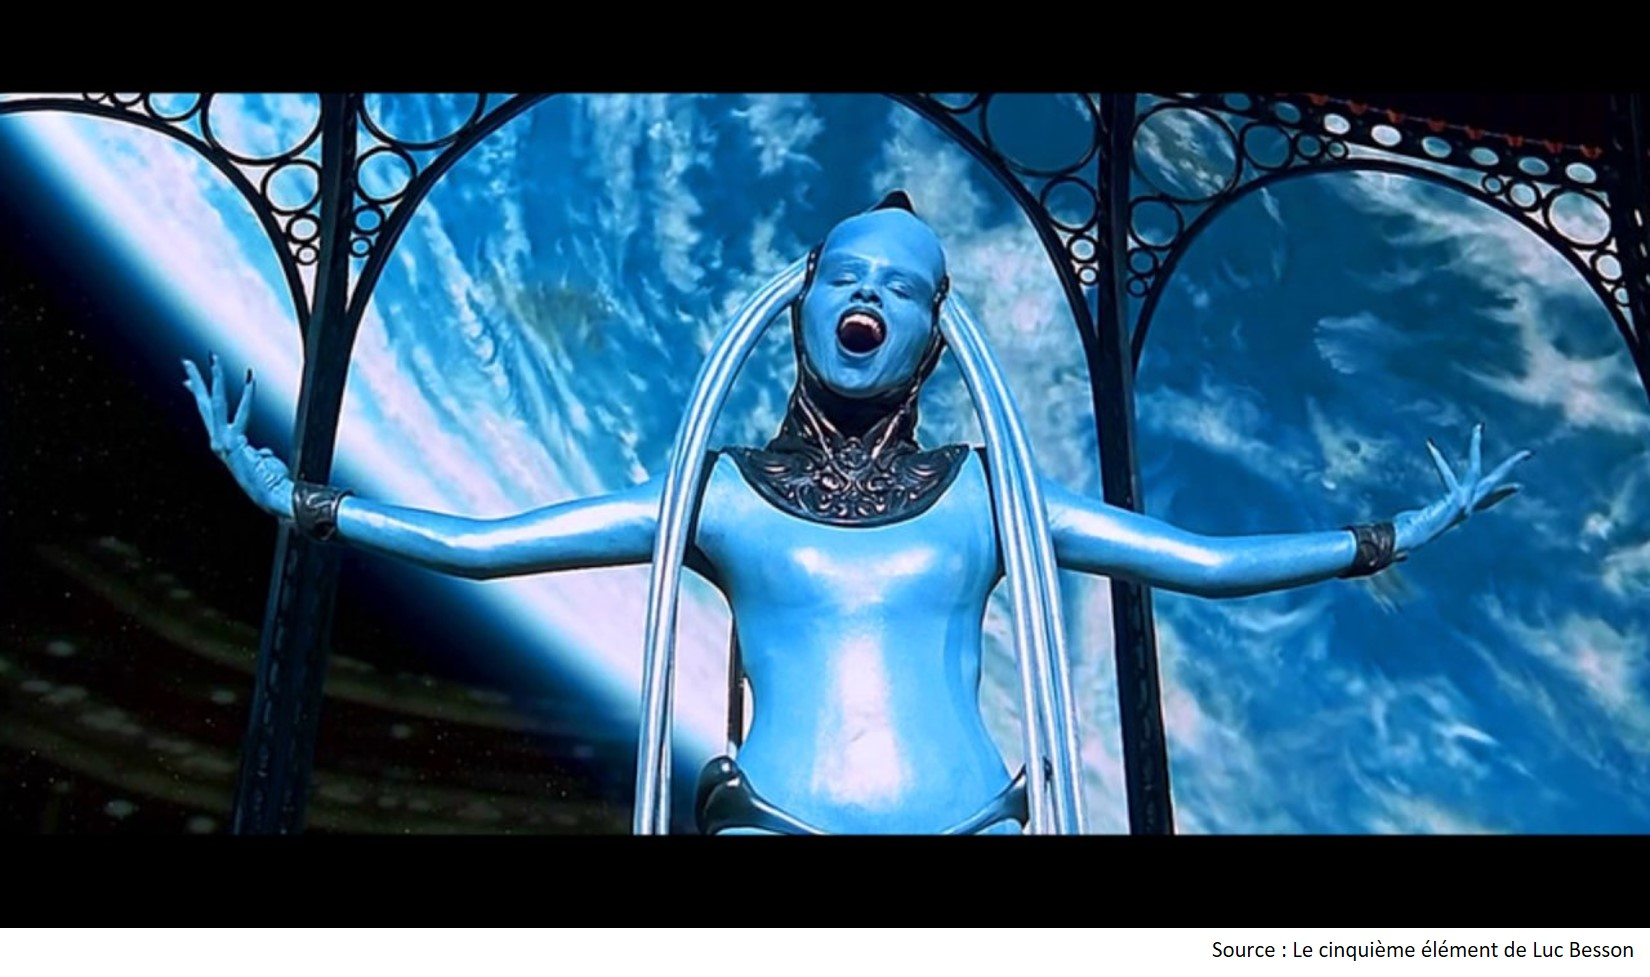
\includegraphics[width=0.4\textwidth]{Images/TP/TP8/Cinquieme_element.jpg}
   \end{wrapfigure}
Inva Mulla-Tchako est une soprano albanaise qui chante régulièrement les premiers rôles dans les plus grands opéras du monde.\\
Dans le film de science-fiction \textit{Le Cinquième élément} réalisé par Luc Besson en 1997, elle prête sa voix au personnage de la diva Plava-Laguna. Éric Serra, le compositeur de la bande originale du film, a déclaré que la voix représentait 85\% de l'enregistrement et que le reste avait dû être travaillé numériquement. Il a aussi déclaré qu'il n'imaginait pas quelqu'un capable de chanter plus de 60\% de la chanson.\\

\problematique{Comment décrire un son ? Comment le visualiser ? Quels outils peut-on utiliser pour déterminer ses propriétés ?}
\end{tcolorbox}


\begin{mdframed}[style=autreexo]
\textbf{\bsc{Liste du matériel}}
\begin{itemize}
    \item Un microphone relié à un ordinateur ;
    \item Un ordinateur muni du logiciel d'enregistrement numérique Audacity ;
    \item Un diapason ;
    \item Une guitare ;
    \item Un ukulele ;
    \item Un accordeur ;
\end{itemize}
\end{mdframed}
 
%%%%
\newpage

\section{Visualisation du son émis par un diapason}
%%%% documents

%%%%
\begin{doc}{Le diapason}
\begin{center}
\vspace{-0.5cm}
     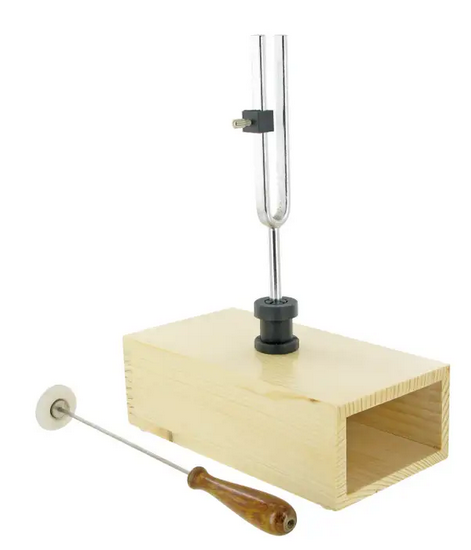
\includegraphics[scale=0.5]{Images/TP/TP8/Diapason.PNG}
\end{center}
Un diapason est constitué de deux branches métalliques parallèles formant un \og U \fg. En vibrant, les branches du diapason émettent un son à une fréquence étalonnée unique : ce son constitue une note de référence mondialement acceptée et notée La3 de fréquence 440~Hz. Cette référence permet aux musiciens d'accorder leurs instruments de musique.\\
Le support en bois du diapason sert de \textcolor{red}{caisse de résonance} c'est-à-dire à amplifier le son émis par le diapason.
\end{doc}

\begin{doc}{Période et fréquence d'un signal périodique}
\begin{tcolorbox}
[colback=green!5!white,colframe=green!75!black,title=\textbf{Signal périodique :}]
Un signal sonore \textcolor{red}{périodique} est un signal qui se \textcolor{red}{reproduit à l'identique} au cours du temps.
\begin{center}
    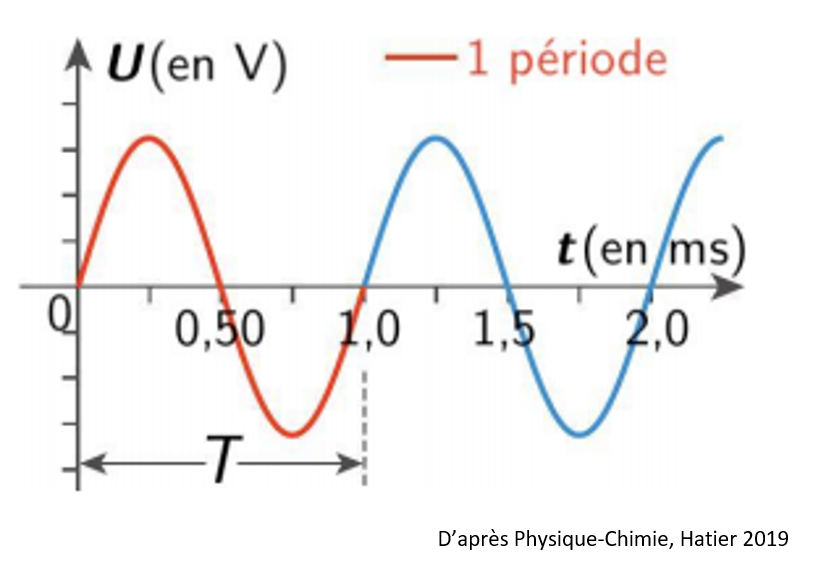
\includegraphics[scale=0.35]{Images/Cours/Chapitre_3/Periode.PNG}
\end{center}
On appelle \textcolor{red}{période}, la plus petite durée au bout de laquelle le signal se répète. On note cette grandeur T et elle s'exprime en seconde (s).
\end{tcolorbox}
\begin{tcolorbox}
[colback=green!5!white,colframe=green!75!black,title=\textbf{Fréquence d'un son :}]
La \textcolor{red}{fréquence}, notée $f$, représente le nombre de périodes d'un signal périodique en 1 seconde. Elle se calcule de la manière suivante : 
\begin{empheq}[box=\fbox]{equation*}
    f = \frac{1}{T}
\end{empheq}
Elle s'exprime en Hz (Hertz) ou s$^{-1}$.
\end{tcolorbox}
\end{doc}

\begin{doc}{Protocole d'utilisation du logiciel Audacity}
\vspace{-1cm}
\begin{wrapfigure}{r}{0.15\textwidth}
\vspace{-0.6cm}
    \centering
     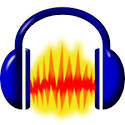
\includegraphics[width=0.15\textwidth]{Images/TP/TP8/Audacity_icone.jpeg}
   \end{wrapfigure}
\begin{enumerate}
    \item Brancher votre micro sur l'entrée jack de l'ordinateur,
    \item Double-cliquer sur l'icône Audacity sur le bureau,
    \item Vous devriez voir l'écran avec la barre de contrôle suivante :
        \begin{center}
        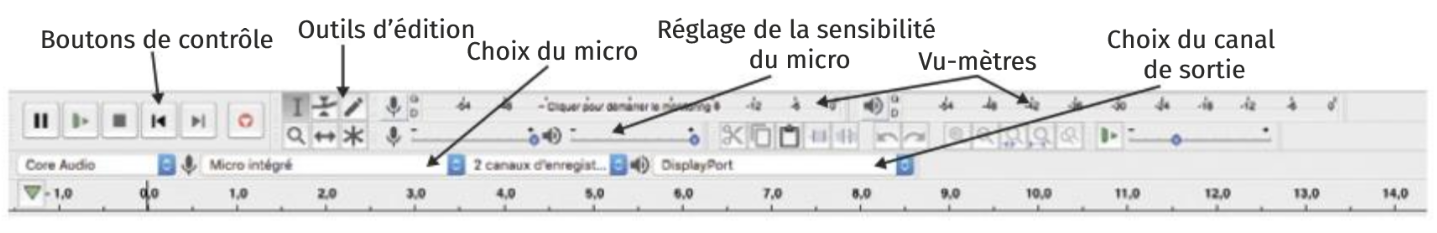
\includegraphics[scale=0.6]{Images/TP/TP8/Audacity.PNG}
        \end{center}
    \item Vérifier que le micro que vous avez branché apparaît dans le choix du micro, sinon appeler le professeur,
    \item Lorsque vous avez enregistré un signal avec les boutons de contrôle, on peut sélectionner une partie avec le click droit de la souris et appuyer sur la \og loupe \fg~ pour zoomer sur le signal. Le curseur vous indique le temps du début et de fin de la partie du signal sonore sélectionnée :
    \begin{center}
        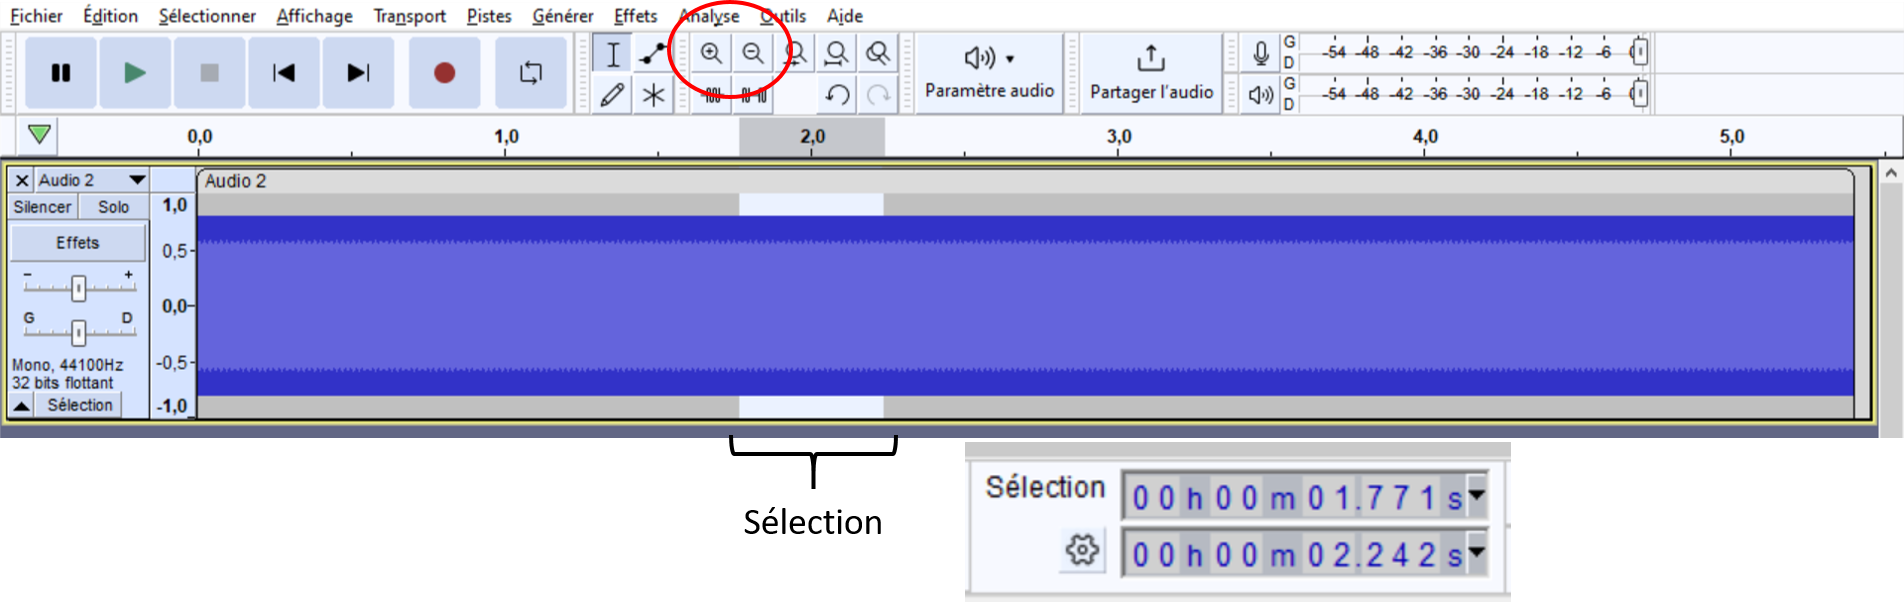
\includegraphics[scale=0.5]{Images/TP/TP8/Audacity_son.png}
    \end{center}
    
\end{enumerate}

\end{doc}
%%%%
\newpage
\begin{large}
    \textbf{\textcolor{red}{\underline{Travail à réaliser :}}}
\end{large}
\\
\vspace{-0.3cm}
\question{\`{A} l'aide du document 3, enregistrer un signal sonore émis par le diapason. Visualiser le signal obtenu en zoomant sur l'écran si nécessaire.}{~}{0}
%\\
\question{Enregistrez une capture d'écran du signal, imprimez la et collez-la sur votre compte rendu.}{~}{0} 
%\\
\question{\`{A} l'aide du document 2, le signal obtenu est-il périodique ? Représenter une période sur le signal que vous avez imprimé.}{~}{0}
%\\
\renewcommand{\arraystretch}{0.8}
\question{\`{A} l'aide des curseurs sur le logiciel Audacity, compléter le tableau suivant :
\begin{center}
\begin{tabular}{|c|C{0.15}|C{0.15}|C{0.15}|C{0.15}|}
    \hline
    Nombre de période & 1 & 5 & 10 & 20 \\
    \hline
    Durée totale (en s) & & & & \\
    \hline
     Période T mesurée (en s) & & & & \\
    \hline
    Fréquence (en Hz) & & & & \\
    \hline
\end{tabular}
\end{center}}{~}{0}
%\\
\question{En déduire la méthode à utiliser pour mesurer une période de façon précise.}{Il faut mesurer le temps entre plusieurs périodes et ensuite diviser le résultat par le nombre de périodes. Cela donne une mesure pour la période plus précise.}{0}
%\\
\question{La fréquence que vous avez mesurée correspond t-elle à celle donnée sur le diapason ?}{Oui, lorsqu'on prend 20 périodes, on obtient une mesure assez précise de la fréquence qui est celle (ou très proche) du diapason.}{0}

\section{Accorder d'une guitare}

\begin{doc}{Quelques notes et fréquences}
\begin{center}
    \begin{tabular}{|c|c|c|c|c|c|c|c|c|}
        \hline
        \cellcolor{orange!25} Note/Octave & Do3 & Ré3 & Mi3 & Fa3 & Sol3 & La3 & Si3 & Do4\\
        \hline 
        \cellcolor{orange!25} Fréquence (en Hz) & 262 & 294 & 330 & 349 & 392 & 440 & 494 & 524 \\
        \hline 
    \end{tabular}
\end{center}
\end{doc}

\begin{large}
    \textbf{\textcolor{red}{\underline{Travail à réaliser :}}}
\end{large}
\\
\question{Comparer l'épaisseur de la corde de guitare et la \textcolor{red}{hauteur} (aigüe ou grave) de la note obtenue en la faisant vibrer.}{Plus l'épaisseur de la corde est importante, plus la note est grave.}{0}
%\\
\question{Afin de comparer leur fréquence, enregistrer et imprimer un son grave et un son aïgu sur une durée totale de 100~ms. Vous imprimerez puis collerez vos signaux sonores sur votre compte-rendu. \textbf{N'oubliez pas d'annoter vos signaux pour ne pas les confondre !}}{~}{0}
%\\
\question{Comparer les deux signaux entre eux (période et fréquence).}{Le son le plus grave à la fréquence la plus basse. Le son le plus aigu a la fréquence la plus grande.}{0}
%\\
\question{D’après le document, quelle est la relation de fréquence entre 2 notes séparées d’une octave ?}{La fréquence entre 2 notes séparées d'une octave est $524-262=262$~Hz.}{0}
\question{\textbf{\underline{Pour les guitare-héros}}, accorder la deuxième corde la plus grave de la guitare pour obtenir la note La3 du diapason. Noter le protocole expérimental que vous mettez en place.}{~}{0}
%\\